\section{MenuView}

Im Menu-View werden alle verfügbaren Menüs, die im \nameref{menucontroller}-Controller gespeichert
sind, in Form einer Liste bestehend aus \lstinline{Card}-Widgets angezeigt.

\subsection{Render-Widget für Menü-Informationen}

Damit ein Nutzer schnell einen Überblick über alle verfügbaren Menüs des Anbieters erhält,
werden alle relevanten Informationen eines jeweiligen Menüs, beispielsweise die inkludierten
Produkte oder der Preis, in einem individualisierten \lstinline{Card}-Widget dargestellt.

Hierfür muss dem Menu-Card-Konstruktor ein Objekt der Menü-Klasse übergeben werden. Aus diesem
werden in der \lstinline{build()}-Funktion des Custom-Widgets alle Daten ausgelesen und in 
entsprechend weiteren Widgets angezeigt.

So befinden sich folgende Inhalte eines Menüs auf dessen Menu-Card:

\begin{itemize}
    \item der Name des Menüs als Titel des Card-Widgets
    \item das Bild des Menüs
    \item alle inkludierten Produkte, welche als Liste angeführt werden
    \item der Preis des Menüs
\end{itemize}

Unter eben genannten Informationen befindet sich ein Button, der auf Druck das entsprechende Menü
zum Warenkorb des Nutzers hinzufügt und zum Kauf bereit macht.

\begin{figure}[H]
    \centering
    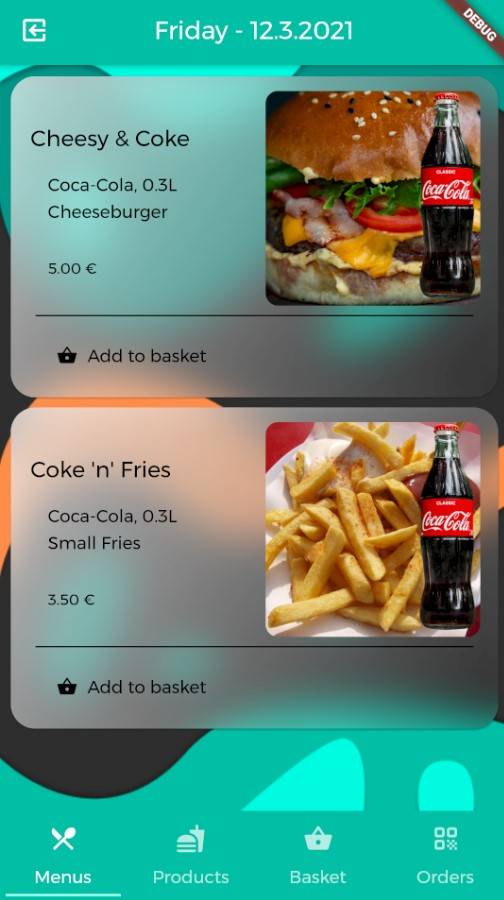
\includegraphics[width=0.40\textwidth]{images/Client/views/menuview/menuView.png}
    \caption{Menu-View mit darauf abgebildeten Menu-Cards}
\end{figure}

\subsection{Rendern der Menu-Cards für alle verfügbaren Menüs}

Um für jedes bestellbare Menü eine solche Menu-Card im eigentlichen View anzuzeigen
wird das \lstinline{ListView.builder}-Widget verwendet.

Dieses Widget erzeugt eine Liste mit einer definierten Anzahl, in unserem Fall
die Anzahl an Menü-Objekten im Menu-Controller, des übergebenen Child-Elements.

\begin{code}[H]
    \centering
    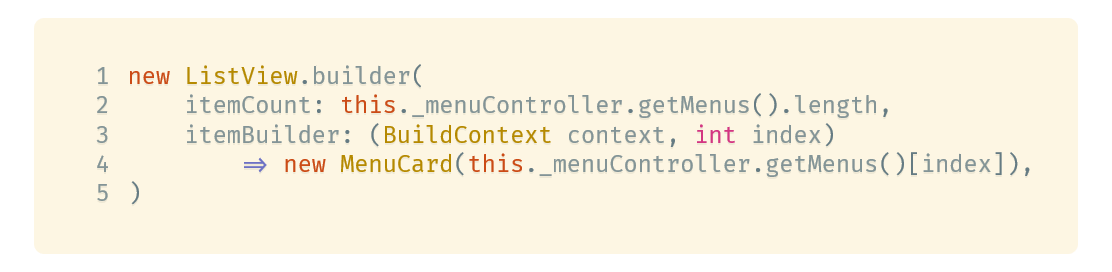
\includegraphics[width=1\textwidth]{images/Client/views/menuview/menuListViewBuilder.png}
    \vspace{-25pt}
    \caption{ListView.builder-Widget zum Erzeugen und Darstellen aller Menu-Cards}
\end{code}

\newpage